%%%%%%%%%%%%%%%%%%%%%%%%%%%%%%%%%%%%%%%%%%%%%%%%%%%%%%%%%%%%%%%%%%%%%%%%%%%%%%%%%%%%%%%%%%%%%
%%									Chapitre 4												%
%%%%%%%%%%%%%%%%%%%%%%%%%%%%%%%%%%%%%%%%%%%%%%%%%%%%%%%%%%%%%%%%%%%%%%%%%%%%%%%%%%%%%%%%%%%%%

\chapter{Calcul de Best Matching Unit accéléré avec la topologie}
	\citationChap{
	Il semble que la perfection soit atteinte non quand il n'y a plus rien à ajouter, mais quand il n'y a plus rien à retrancher.
	}{Antoine de Saint-Exupéry}
	\minitoc
	\newpage

%%%%%%%%%%%%%%%%%%%%%%%%%%%%%%%%%%%%%%%%%%%%%%%%%%%%%%%%%%%%%%%%%%%%%%%%%%%%%%%%%%%%%%%%%%%%%



% Début du chapitre			
	\section{Introduction}

	Self-Organizing Maps (SOM) are well-known unsupervised neural networks able to perform vector quantization while mapping an underlying regular neighbourhood structure onto the codebook. They are used in a wide range of applications. As with most properly trained neural networks models, increasing the number of neurons in a SOM leads to better results or new emerging properties. Therefore highly efficient algorithms for learning and evaluation are key to improve the performance of such models. In this paper, we propose a faster alternative to compute the Winner Takes All component of SOM that scales better with a large number of neurons. We present our algorithm to find the so-called best matching unit (BMU) in a SOM, and we theoretically analyze its computational complexity. Statistical results on various synthetic and real-world datasets confirm this analysis and show an even more significant improvement in computing time with a minimal degradation of performance. With our method, we explore a new approach for optimizing SOM that can be combined with other optimization methods commonly used in these models for an even faster computation in both learning and recall phases.

	Self-organizing maps (SOM) are widely used algorithms that feature vector quantization with dimensionality reduction properties. An explanation of how they work can be found in \cite{kohonen2007kohonen}. They are used in numerous fields like image processing, automatic text and language processing, and for visualization, analysis and classification of all kinds of highly dimensional datasets. Many applications examples are depicted in \cite{cottrell:hal-01796059}. However, the amount of computations required by SOMs linearly increases with the number of neurons, the number of elements in the dataset and the dimensionality of the input, in both learning and recall phases. Therefore applying SOMs on datasets with huge numbers of elements and with a high number of neurons to precisely represent the input induces a significant computational cost that may exceed some constraints such as real-time computation or low power consumption.

	With the goal of reducing the required computational time of SOMs in mind, variants of the classical SOM algorithm have been developed. The most well-known SOM modification is the Batch Learning algorithm, as explained in  \cite{cottrell:hal-01796059}. Contrary to the classical online learning, the batch learning averages the modifications over multiple training vectors before updating the neurons weights. Similar efforts have been made in \cite{fiannaca2013simulated} or in \cite{oyana2012new}. However, all those variants are only focusing on reducing the convergence time of the SOM training. To the best of our knowledge, no work has been carried out to reduce the time required for each iteration. This can be partially explained by the highly parallel nature of the computations inside each iterations, in so far as when a fast real world implementation is required, parallel solutions are proposed, like the use of an FPGA substrate with each neuron having its own circuitry, as in \cite{abadi2018scalable} and in \cite{huang2017hardware}. However, parallel solutions should not lead to a lack of effort in optimizing the algorithms, as the majority of SOM training is performed on CPU, and parallel hardware can be costly and difficult to program. Furthermore one can parallelise multiple iterations within an epoch instead of inside the iteration itself, and therefore can benefit from our improvements on parallel hardware.

% -- ICANN Version --
	A SOM training iteration consists of two major parts, a competitive part which searches the Best Matching Unit (or winner neuron), and a cooperative part which updates all the neurons weights proportionally to their distance with the BMU. In the classic SOM, both steps have the same algorithmic complexity (number of neurons multiplied by the dimensionality of the data) and take roughly the same time (depending on implementation details). In this paper we focus on improving the competitive part by reducing the number of neurons evaluated to find the BMU. This optimization also applies to the recall phase.

% -- IJCAI VERSION -- A SOM iteration is composed of two steps during training. The first step consists in finding the Best Matching Unit (or winner neuron), which is done with a comparison between the input vector and the weight vectors of all neurons. The second step consists in modifying the weights of each neuron with regard to its neural distance to the Best Matching Unit. In the classic SOM algorithm, the two steps have the same algorithmic complexity (number of neurons multiplied by the dimensionality of the data) and take roughly the same time (depending on implementation details). In this paper we focus on improving the first step of an iteration by reducing the number of comparisons required to find the Best Matching Unit (BMU). This optimization also applies to the recall phase that reduces to the first step for each new input pattern.

	After a brief description of the standard SOM model in section \ref{seq:som}, section \ref{seq:algorithm} defines the proposed method to speed up the computation of BMU, before analyzing its computational complexity. The experimental setup is described in section \ref{seq:exp_setup}, 
%including various datasets and the definition of the associated performance measures. 
	and the corresponding results are discussed in section \ref{seq:results}.

	We present here our new algorithm for searching the Best Matching Unit (BMU) in the SOM. It is traditionally determined by means of an exhaustive search by comparing all the distances between the input vector and the neurons weights. This method, while able to always find the correct minimum of the map, is computationally inefficient. The dimensionality reduction property of the SOM means that close neurons in the SOM topology represent close vectors in the input space. Therefore when an input vector is presented to the SOM, a pseudo-continuous gradient appears in the SOM when considering the distances between the neuron weights and the input vector whose minimum is located at the BMU. Using some kind of discretized gradient descent approach, we expect that this distance will progressively reduce until the Best Matching Unit is reached, with the minimal distance in the map. 

	\newpage

	\section{Algorithme séquentiel}

	Pour bien comprendre le fonctionnement de notre algorithme Fast-BMU, nous allons le présenter partie par partie. Nous commencerons par l'idée générale de la descente du gradient de la SOM. Puis nous aborderons les cas spéciaux en expliquant pourquoi ils existent, les conséquences possibles et comment Fast-BMU les résoud.

	\begin{algorithm}
	\caption{Particule}
	\label{fast:alg:particle}
	\DontPrintSemicolon
	\Entree{\;
	{\tt vecteur} : vecteur d'entrée \;
	{\tt pos}: position de la particule}
	\Donnees{\;
	{\tt memoire\_dist}: historique des distances déjà évaluées\;}
	\Sortie{\;
	{\tt bmu} : index de la Best Matching Unit potentielle\;\;}

	\Deb{
		\tcp{On commence par regarder les voisins directs pour trouver si l'un}
		\tcp{d'entre eux est plus proche du vecteur d'entrée.}
		{\tt bmu\_voisin} $\leftarrow$ RechercheVoisin({\tt vecteur}, {\tt pos}, 1)\;
		\Si{{\tt memoire\_dist[bmu\_voisin]} $<$ {\tt memoire\_dist[\tt pos]}}{
			\Retour{Particule({\tt vecteur}, {\tt bmu\_voisin})}
		}
		\tcp{Si il n'y en a pas, alors on se trouve dans un minimum local.}
		\tcp{On effectue alors une nouvelle recherche dans le voisinage de 2.}
		{\tt bmu\_voisin} $\leftarrow$ RechercheVoisin({\tt vecteur}, {\tt pos}, 2)\;
		\Si{{\tt memoire\_dist[bmu\_voisin]} $<$ {\tt memoire\_dist[\tt pos]}}{
			\Retour{Particule({\tt vecteur}, {\tt bmu\_voisin})}
		}
		\tcp{Si on ne trouve toujours rien, alors on peut considérer que l'on a atteint}
		\tcp{la fin de la descente de gradient.}
		\Retour{{\tt pos}}
	}
	\end{algorithm}

	\begin{algorithm}
	\caption{RechercheVoisin}
	\label{fast:alg:voisin}
	\DontPrintSemicolon
	\Entree{\;
	{\tt vecteur} : vecteur d'entrée \;
	{\tt pos}: position de la particule\;
	{\tt x}: distance topologique}
	\Donnees{\;
	{\tt resultats}: dictionnaire vide\;
	{\tt prototypes}: valeurs des vecteurs prototypes de la SOM\;
	{\tt memoire\_dist}: historique des distances déjà évaluées\;}
	\Sortie{\;
	{\tt bmu} : index de la Best Matching Unit potentielle\;\;}

	\Deb{
		\Pour{{\tt voisin} dans le voisinage à distance topologique x de {\tt pos}}{
			\Si{{\tt memoire\_dist[voisin]} est vide}{
				{\tt memoire\_dist[voisin]} $\leftarrow$ distance({\tt prototypes[voisin]}, {\tt vecteur})\;
				{\tt resultats[\tt voisin]} $\leftarrow$ {\tt memoire\_dist[voisin]}\;
			}
		}
		{\tt bmu\_voisin} $\leftarrow$ minimum de {\tt resultats} par valeurs\;
		\Retour{{\tt bmu\_voisin}}
	}
	\end{algorithm}

	Le coeur de Fast-BMU est la descente de gradient discrétisée sur les neurones qui minimise la distance entre ceux-ci et le vecteur d'entrée. Le pseudo-code de cette descente de gradient, appelée \textit{Particule}, est présenté dans les algorithmes \ref{fast:alg:particle} et \ref{fast:alg:voisin}. Une \textit{Particule} commence à une position choisie arbitrairement dans la carte. Pour cet exemple, illustré dans la figure \ref{fig:first_particle}, considérons qu'elle débute aux coordonnées $(0,0)$ (coin supérieur gauche). Ce neurone a deux voisins, un à l'est (1,0) et un au sud (0,1). Nous évaluons les distances au vecteur d'entrée de ces trois neurones pour trouver la prochaine étape de la descente du gradient. Si l'un des neurones voisins donne la plus petite distance, alors la descente du gradient va dans la direction de ce neurone particulier, qui devient la prochaine position sélectionnée à partir de laquelle nous répétons ce processus. Si la plus petite distance est trouvée là où nous sommes actuellement positionnés, alors nous considérons que nous nous trouvons dans un minimum local. Dans notre exemple, la plus petite distance est mesurée pour le neurone situé à l'est en (1,0). Le processus de recherche se déplace donc d'un pas vers l'est. Ce neurone a trois voisins, un au sud (1,1), un à l'est (2,0) et un à l'ouest dont nous venons et que nous allons donc ignorer. Nous comparons à nouveau les trois distances et nous nous déplaçons vers la distance la plus faible (le Sud). Ce processus itère jusqu'à atteindre un minimum local à la position (6,5), où tous les neurones voisins ont une distance au vecteur d'entrée plus élevée que le neurone sélectionné.

	Trouver un neurones sans meilleurs voisins ne garantit cependant pas que l'on a terminé la descente de gradient. On peut observer par exemple sur la figure \ref{fig:first_particle} que les neurones au sud et à l'ouest du premier minimum local ont un gradient qui pointent vers un autre neurone que le minimum local actuel. Cela s'explique par le fait que, surtout pour les topologies en grille, le gradient soit en diagonale, et que par conséquent qu'il faille deux étapes (sud puis ouest ou ouest puis sud) continuer la descente. Pour compenser ce problème, et afin de s'assurer que le minimum local qui a été trouvé est bien le meilleur dans le voisinage local, nous effectuons une recherche de minimum dans tous les voisins à voisinage topologique de 2. Si un nouveau minimum a été trouvé, nous continuons la descente de gradient à partir de celui-ci. Si il n'y en a pas, alors nous considérons que la descente de gradient est terminée, et que la position actuelle est le minimum trouvé. Car tous ses voisins sont moins bons, et que le gradient de tous ses voisins amènent à lui.

	\begin{figure}[!t]
    	\centering
    	\includesvg[scale=1.2]{first_particle}\ \ \ \ \ \ \ 
    	\includesvg[scale=1.2]{all_particles}
		\caption[Visualisation de l'algorithme de particule]{À Gauche : exemple d'exécution d'une particule. Chaque cellule représente un neurone. La flèche dans chaque cellule pointe vers le meilleur voisin (qui a une distance inférieure). Une étoile représente un minimum local. Les cellules vertes sont les neurones qui ont été explorés pendant la recherche, et les cellules bleues sont les neurones dont la distance au vecteur d'entrée a été calculée mais qui n'ont pas été sélectionnés par l'algorithme. Après avoir trouvé un minimum local, de nouvelles particules sont créées (en rouge) et continuent la descente du gradient en explorant le voisinage local. La cellule en jaune est la BMU, et le minimum global de la carte. À droite : exécution des quatre particules.}
    	\label{fig:first_particle}
	\end{figure}

	Un autre problème qui peut survenir avec une unique \textit{Particule} est dû aux bords. Lors du mappage de données à haute dimension sur une SOM 2D, la carte peut parfois devenir tordue sans gradient continu entre le neurone supérieur gauche et le neurone inférieur droit. Imaginez par exemple un filet que l'on jette sur une sphère et qui l'enveloppe presque complètement : le chemin le plus court entre un coin du filet et le coin opposé du filet ne suivra pas les mailles du filet. Si, au cours de la phase d'apprentissage, la particule se retrouve dans le mauvais coin de la SOM, elle trouvera une très mauvaise BMU et la mise à jour des vecteurs prototypes des neurones brisera localement la continuité du voisinage, et créera une boucle de rétroaction négative qui détruira toutes les propriétés de réduction dimensionnelles de la SOM. Il existe un moyen facile d'éviter cela, en démarrant 4 \textit{Particules}, une dans chaque coin de la SOM, et en sélectionnant la plus petite BMU trouvée parmi les 4. Cette technique préserve la continuité du SOM et rend l'algorithme Fast-BMU plus robuste aux discontinuités locales du gradient, notamment au début de l'apprentissage, lorsque la carte n'est pas encore bien déployée. Fast-BMU complet est défini dans l'algorithme \ref{fast:alg:bmu}, et le résultat d'une exécution complète est illustré dans la figure \ref{fig:first_particle} à droite.
	
	Il faut aussi remarquer que dans le cas où il n'y a pas de gradient clair dans la SOM (typiquement lorsque la SOM est initialisée de façon aléatoire avant l'apprentissage), Fast-BMU ne trouvera pas la BMU correcte. Toutefois, ce n'est pas un problème pour l'apprentissage, car la fonction de voisinage créera un gradient en dépliant la SOM, quel que soit le neurone initialement sélectionné, et une fois le gradient créé, Fast-BMU trouvera les bonnes BMU.

	\begin{algorithm}
	\caption{FastBMU}
	\label{fast:alg:bmu}
	\DontPrintSemicolon
	\Entree{\;
	{\tt vecteur} : vecteur d'entrée \;
	{\tt l, h}: largeur et hauteur de la SOM}
	\Donnees{\;
	{\tt positions}: positions de départ des particules\;
	{\tt memoire\_dist}: historique des distances déjà évaluées\;
	{\tt resultats}: dictionnaire vide}
	\Sortie{\;
	{\tt bmu} : index de la Best Matching Unit\;\;}

	\Deb{
		{\tt positions} $\leftarrow [(0,0), (l-1, 0), (0, h-1), (l-1, h-1)]$\;
		\Pour{{\tt pos} dans {\tt positions}}{
			{\tt bmu\_particule} = Particule({\tt vector}, {\tt pos})\;
			{\tt resultats[bmu\_particule]} $\leftarrow$ {\tt memoire\_dist[bmu\_particule]}\;
		}
		{\tt bmu} = minimum de {\tt resultats} par valeurs\;
		\Retour{{\tt bmu}}
	}
	\end{algorithm}

	\subsection{Analyse de la complexité}\label{seq:complex_analysis}

	Le temps d'exécution d'une recherche de BMU dans la SOM classique dépend de deux facteurs : le nombre de neurones multiplié par la durée d'une comparaison entre le vecteur d'entrée et les poids d'un neurone. L'idée de Fast-BMU étant de réduire le nombre de ces comparaisons, la durée d'une comparaison ne sera pas prise en compte dans cette analyse. C'est normalement une valeur constante qui ne dépend que de la dimensionalité des données. Le nombre de comparaisons pour Fast-BMU est quand à lui dépendant de la taille de la carte, c'est à dire hauteur et largeur, et de la topologie, c'est à dire du nombre de voisins par neurone. 

	Nous ferons dans cette analyse l'hypothèse qu'il y a une certaine continuité dans la carte et qu'en partant de n'importe quel point de la carte, on atteigne la BMU en suivant le gradient. C'est une hypothèse forte, mais qui doit être vraie pour que notre algorithme de Fast-BMU fonctionne. En pratique, Fast-BMU est plus robuste que cela, et n'a pas besoin que tous les gradients de la carte mènent à la BMU, il en faut juste assez pour qu'une \textit{particule} la trouve. De plus, les problèmes les plus communs dans le gradient de la carte sont des minimums locaux, qui réduisent le nombre de \textit{pas} en arrêtant la \textit{particule} avant la fin. Pour augmenter le nombre de pas effectués par une particule, il faudrait un gradient qui prenne une direction à l'opposé de ce qu'il avait précédemment. Qu'il fasse des méandres sur son trajet par exemple, ce qui est inhabituel dans des SOM en général. Ainsi, la complexité que nous allons calculer sera probablement une limite haute à la vraie complexité de l'algorithme Fast-BMU. 

	Pour estimer la complexité de notre algorithme, c'est à dire le nombre de comparaisons dans notre cas, nous devons estimer le nombre de \textit{pas} de chaque particule pour trouver la BMU potentielle. En considérant que la BMU est localisée à la position $x, y$ de la SOM, on a :
	\begin{itemize}
    	\item La \textit{particule} en haut à gauche commençant aux coordonnées $0, 0$ devra faire $x$ \textit{pas} horizontaux et $y$ \textit{pas} verticaux pour atteindre la BMU.
		\item De la même façon, la \textit{particule} du haut à droite avec les coordonnées $(w,0)$ devra faire $w-x$ \textit{pas} horizontaux et $y$ pas verticaux.
		\item Pour la \textit{particule} en bas à gauche $(0,h)$, ce sera $x$ et $h-y$ \textit{pas}.
		\item Pour la \textit{particule} en bas à droite $(w,h)$, ce sera $w-x$ et $h-y$ \textit{pas}.
	\end{itemize}

	Pour obtenir le nombre total de \textit{pas} pour une itération, nous additionons les nombres de pas de toutes les particules ensemble comme montré dans l'équation \ref{fast:eq:nbsteps}.

	\begin{equation}\label{fast:eq:nbsteps}
	\begin{split}
    	\text{NbrPas} &= (x + y) + (w - x + y) + (x + h - y) + (w - x + h - y)\\
		&= 2x - 2x + 2y - 2y + 2w + 2h 
	\end{split}
	\end{equation}

	Les $x$ et $y$ s'annulant, le nombre total de pas ne dépend donc que de la largeur et la hauteur de la carte, soit $(2w + 2h)$. On peut donc en déduire la Complexité Estimée $\cal C$ avec l'équation \ref{fast:eq:complexity}

	\begin{align}\label{fast:eq:complexity}
    	{\cal C}(w, h) = 2 \times (w + h) \times \textit{NbrEvalParPas}
	\end{align}

	avec $w, h$ la largeur et la hauteur de la SOM respectivement et \textit{NbrEvalParPas} le nombre de nouvelles distances à calculer pour chaque \textit{pas} d'une particule. Sa valeur dépend de la topologie. Elle est au maximum de 3 avec une grille (4 voisins moins le neurone de l'étape précédente) et également de 3 avec une topologie hexagonale (6 voisins moins le neurone de l'étape précédente et 2 neurones qui étaient voisins du neurone précédent et qui ont donc déjà été évalués). 

	D'un point de vue analytique, nous pouvons estimer que notre algorithme Fast-BMU (${\cal C}(w,h)=6(w+h)$ dans le pire des cas dans une configuration de grille standard) est significativement plus rapide que l'algorithme actuel de recherche exhaustive (O$(w,h) = wh$) lorsque le nombre de neurones dans la carte est important. Par exemple, il est théoriquement deux fois plus rapide avec des SOM de 24 par 24, et 10 fois plus rapide avec des SOM de 120 par 120. Une évaluation expérimentale de la différence de vitesse est présentée dans la section \ref{fast:seq:gain_comput}.

	\subsection{Protocole expérimental}\label{seq:exp}

	Pour évaluer la robustesse de notre algorithme avec différents types de données, nous avons sélectionné 6 jeux de données représentatifs du type de données sur lesquelles les SOM sont habituellement entraînés. Pour le cas 2D, nous avons généré des données avec différentes propriétés (une distribution uniforme et une forme hautement non convexe), pour les données 3D nous utilisons une forme cubique uniformément distribuée et les valeurs de couleur des pixels d'une image. Pour les hautes dimensions, nous considérons l'apprentissage par imagettes d'une image déjà présenté, avec des sous-images de 10 par 10 comme vecteurs d'entraînement (100 pixels avec 3 couleurs chacun, ce qui donne 300 dimensions), ainsi que le Free Spoken Digits Dataset \cite{zohar_jackson_2018_1342401} qui utilise des ondes sonores que nous avons réduites à 1000 dimensions. Nous emploierons des SOM à 2 dimensions avec des topologies en grille et hexagonales, car ce sont les plus utilisées.

	Pour ces tests, nous avons fait débuter $\alpha$ à 0.6 pour finir à 0.05. $\sigma$ commence à 0.5 et termine à 0.001. La SOM est de taille $32\times32$ (1024 neurones) et apprend pendant 10 époques.

	Afin d'évaluer les différences entre tous les modèles testés, nous avons utilisé deux métriques. La première est la \textit{Mean Squared Quantization Error} (MSQE) que nous avons déjà utilisée dans le chapitre 2. MSQE mesure la qualité de quantification vectorielle de l'algorithme testé. La seconde métrique est la \textit{Mean Squared Distance to Neurons} (MSDtN) qui calcule la distance moyenne au carré entre les prototypes des neurones et ceux de leurs voisins directs. Plus cette valeur est faible, plus les neurones voisins sont proches dans l'espace d'entrée et plus la propriété de réduction dimensionnelle est bonne. De nombreuses métriques existent dans la littérature sur les SOM pour la qualité de la réduction dimensionnelle d'une SOM, mais MSDtN a l'avantage d'être facile à calculer, sans paramètres et de ne dépendre que des poids des neurones. Pour toutes les métriques, une valeur plus faible est meilleure. 

	\begin{equation}
		\text{MSQE} = \frac{1}{dn} \sum_{i=0}^{n-1} (v_i - u_i)^2
	\end{equation}

	\begin{equation}
    	\text{MSDtN} = \frac{1}{dN} \sum_{i=1}^{N} \sum_{j=1}^{N} 
    	\begin{cases}
        	(w_i - w_j)^2,  & \text{Si dist}(i, j) = 1\\
        	0,              & \text{Sinon}
    	\end{cases}
	\end{equation}

	Avec $n$ étant le nombre de vecteurs dans le jeu de données, $d$ leur dimensionalité, $v_i$ les poids du $i^{ème}$ vecteur d'entrée, et bmu($i$) l'indice du neurone qui est la \textit{best matching unit} de $v_i$. De même, $N$ est le nombre de neurones de la SOM et $w_i$ les poids du $i^{ème}$ neurone, tandis que dist($i, j$) est le nombre de connexions dans le chemin le plus court entre les neurones $i$ et $j$ dans la carte neuronale.

	\subsection{Résultats}
	\subsubsection{Performances}

	Dans cette section, nous examinerons les différences de qualité d'apprentissage et de reconstruction entre la version standard et notre version FastBMU pour le calcul de la BMU. Nous regarderons également les différences pratiques dans le nombre de calculs requis pour les deux versions et nous les comparerons avec l'analyse de complexité présentée précédemment.

	Pour chaque combinaison de jeu de données et de modèle (choix de la topologie et de l'algorithme BMU), nous avons effectué 50 exécutions avec différentes graines aléatoires qui affectent les jeux de données générés, l'initialisation des poids des neurones (qui sont tous initialisés aléatoirement sans gradient préexistant) et l'ordre dans lequel les vecteurs d'apprentissage sont présentés. Les résultats sont présentés dans le tableau \ref{tab:recap:param}.

	La colonne algorithme du tableau indique la combinaison de l'algorithme de recherche de BMU et de la topologie qui a été utilisée pour l'entraînement. La MSDtN (voir section \ref{seq:exp}) est calculée sur les poids des neurones entraînés. La MSQE\_S (Standard) est l'erreur de quantification dans la phase de reconstruction (après apprentissage) en utilisant la recherche de BMU standard. La comparaison des différentes valeurs de MSQE\_S pour des SOM ayant été apprises par une version standard et une version rapide de la recherche de BMU donne une indication de l'influence de l'algorithme Fast-BMU sur la qualité de l'apprentissage uniquement, car il sélectionne toujours la vraie BMU dans la phase de reconstruction. La métrique MSQE\_F (Fast) mesure l'erreur de quantification vectorielle avec la sélection de BMU effectuée par l'algorithme Fast-BMU. Si l'entraînement a été effectué sur la SOM standard, il donne une indication de l'influence de l'algorithme Fast-BMU sur la précision du reconstruction uniquement ; s'il a été entraîné sur une version Fast, il représente le résultat MSQE d'une SOM qui utilise uniquement l'algorithme Fast-BMU. La colonne mismatch donne la proportion de BMU qui sont sélectionnées différemment par les deux algorithmes.

	\begin{tableth}
	\caption[Résultats de FastBMU sur différentes données]{Résultats avec une SOM de $32\times32$ neurones, avec 50 executions par ligne. La colonne \textit{Algorithme} précise avec quel algorithme et quelle topologie la SOM a été entraînée. MSQE\_S est le MSQE calculé après apprentissage avec l'algorithme BMU standard (exhaustif) tandis que MSQE\_F utilise la version Fast-BMU. Nous combinons les deux apprentissages avec les deux reconstructions possibles (Standard et Fast). Les différences de MSQE\_S entre les différents algorithmes reflètent ainsi la qualité de la phase d'apprentissage. Le \textit{Mismatch} est la proportion de BMU qui sont sélectionnés différemment par les deux algorithmes.}
	\begin{tabular}{|c|l|r|r|r|r|}
	\hline
	Données & Algorithme & MSDtN & MSQE\_S & MSQE\_F & Mismatch\\
	\hline
	Carré 	& Grille  & \nbr{1.94e-4} & \nbr{2.22e-4} & \nbr{2.22e-4} & 0\%\\
    (2D)   	& Fast-Grille & \bst{1.93e-4} & \nbr{2.23e-4} & \nbr{2.23e-4} & 0\%\\
        	& Hexagonal	& \nbr{2.39e-4} & \bst{2.12e-4} & \bst{2.12e-4} & 0\%\\
        	& Fast-Hexa	& \nbr{2.38e-4} & \nbr{2.15e-4} & \nbr{2.15e-4} & 0\%\\
	\hline
	Forme   & Grille  & \bst{1.38e-4} & \nbr{1.40e-4} & \nbr{1.40e-4} & $\approx$0\%\\
    (2D)    & Fast-Grille & \bst{1.38e-4} & \nbr{1.40e-4} & \nbr{1.40e-4} & $\approx$0\%\\
        	& Hexagonal   & \nbr{1.65e-4} & \bst{1.31e-4} & \bst{1.31e-4} & $\approx$0\%\\
        	& Fast-Hex & \nbr{1.65e-4} & \bst{1.31e-4} & \bst{1.31e-4} & $\approx$0\%\\
	\hline
	Cube   	& Grille  & \bst{4.48e-4} & \nbr{2.21e-3} & \nbr{2.50e-3} & 4.8\%\\
    (3D)   	& Fast-Grille & \nbr{4.61e-4} & \nbr{2.25e-3} & \nbr{3.21e-3} & 9.8\%\\
        	& Hexagonal   & \nbr{5.29e-4} & \bst{2.09e-3} & \bst{2.34e-3} & \bf{3.1\%}\\
        	& Fast-Hex & \nbr{5.38e-4} & \nbr{2.11e-3} & \nbr{2.79e-3} & 7.6\%\\
	\hline
	Couleurs& Grille  & \bst{1.15e-4} & \nbr{8.64e-5} & \nbr{8.80e-5} & 4.4\%\\
    (3D)    & Fast-Grille & \nbr{1.19e-4} & \nbr{8.91e-5} & \nbr{9.08e-5} & 5.4\%\\
        	& Hexagonal   & \nbr{1.33e-4} & \nbr{8.29e-5} & \nbr{8.30e-5} & \bf{0.4\%}\\
       		& Fast-Hex & \nbr{1.35e-4} & \bst{8.26e-5} & \bst{8.29e-5} & 0.7\%\\
	\hline
	Image  	& Grille  & \bst{1.64e-4} & \nbr{1.80e-3} & \nbr{1.83e-3} & 4.2\%\\
    (300D)    & Fast-Grille & \nbr{1.65e-4} & \nbr{1.82e-3} & \nbr{1.85e-3} & 4.4\%\\
        	& Hexagonal   & \nbr{1.97e-4} & \bst{1.75e-3} & \nbr{1.77e-3} & \bf{1.2\%}\\
        	& Fast-Hex & \nbr{1.99e-4} & \bst{1.75e-3} & \bst{1.76e-3} & \bf{1.2\%}\\
	\hline
	Sons    & Grille  & \nbr{2.02e-4} & \nbr{1.42e-2} & \nbr{1.49e-2} & 31.3\%\\
    (1000D)   	& Fast-Grille & \bst{1.93e-4} & \nbr{1.44e-2} & \nbr{1.51e-2} & 32.2\%\\
        	& Hexagonal   & \nbr{2.29e-4} & \bst{1.41e-2} & \bst{1.45e-2} & 19.8\%\\
        	& Fast-Hex & \nbr{2.25e-4} & \nbr{1.42e-2} & \bst{1.45e-2} & \bf{13.3\%}\\
	\hline
	\label{tab:recap:param}
	\end{tabular}
	\end{tableth}

	Nous observons d'abord que la distance entre les neurones après apprentissage (MSDtN) est plus faible avec la topologie en grille qu'avec la topologie hexagonale, mais cette différence pourrait être attribuée au nombre différent de voisins entre les deux topologies et ne devrait donc être utilisée que pour comparer les différences entre les algorithmes standard et Fast-BMU, et pas les topologies. Nous remarquons également que l'algorithme Fast ne présente pas d'écart significatif sur les jeux de données Square et Shape, et donc que MSQE\_S et MSQE\_F ont des résultats de reconstruction similaires sur ces jeux de données.

	Les pourcentages de \textit{mismatch} varient considérablement d'un ensemble de données à l'autre. De 0 à 6\% pour les jeux de données Images et Couleurs, de 3 à 10\% pour le Cube et de 13 à 33\% pour les données sonores. Ces différences peuvent s'expliquer par la distribution des données d'entrée, car les jeux de données Images et Couleurs contiennent des éléments qui sont étroitement liés entre eux. Dans les images, par exemple, il y a généralement quelques couleurs dominantes avec beaucoup de valeurs intermédiaires qui rendent les continuités de la distribution plus faciles à réduire dimensionnellement pour une SOM, améliorant ainsi les performances de notre algorithme Fast-BMU. En revanche, le jeu de données \textit{Spoken Digits} présente des valeurs de \textit{mismatch} élevées, ce qui semble indiquer qu'une forte continuité dans les poids des neurones n'est pas présente après l'apprentissage. La topologie hexagonale est également plus performante avec l'algorithme Fast-BMU que la topologie en grille, car les \textit{mismatch} sont nettement plus faibles avec elle. Enfin, la dimensionnalité d'un jeu de données ne semble pas jouer un rôle clé ici, puisque le jeu de données Image (300 dimensions) présente moins de \textit{mismatch} que le jeu de données Cube (3 dimensions).

	Pour la partie quantification vectorielle, la topologie hexagonale donne à nouveau les valeurs d'erreur les plus faibles. Ce qui est plus surprenant, c'est que la version Fast-BMU présente des résultats de quantification très similaires à ceux de la version standard. Même avec des \textit{mismatch} élevés (30\% avec Digits utilisant un SOM basé sur une grille), le MSQE n'est supérieur que d'environ 5\%, et encore moins lorsque seul l'apprentissage est comparé. Les seules valeurs de MSQE significativement plus élevées avec Fast-BMU concernent le jeu de données Cube, où l'algorithme sélectionne de très mauvais choix de BMU dans la phase de reconstruction tout en étant capable de former correctement la SOM. Dans la plupart des cas, une différence dans la topologie de la SOM a plus d'impact sur la MSQE que l'utilisation de l'algorithme Fast-BMU.

	\subsubsection{Gain computationnels}\label{fast:seq:gain_comput}

	\begin{figureth}
    	\centering
    	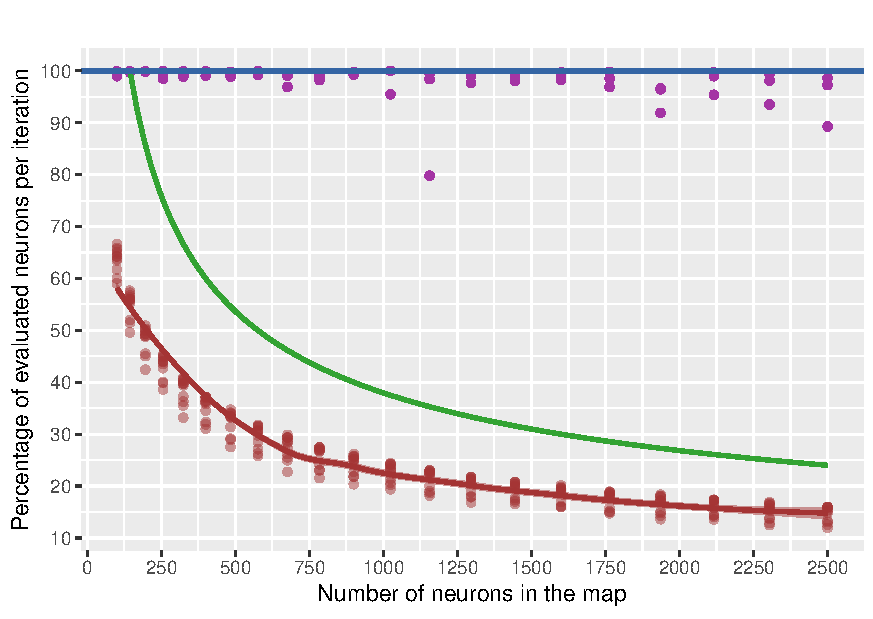
\includegraphics[width=1\textwidth]{performance_diff.pdf}
	%    \includesvg[inkscapelatex=false, width=0.8\textwidth]{performance_diff.pdf}
    	\caption[Évaluation des gains de performance en fonction du nombre de neurones]{Évaluation des gains de performance en fonction du nombre de neurones. Le gain en performance est exprimé en pourcentage de neurones qui ont dû être évalués pendant la recherche de BMU. Tous les résultats ont été calculés sur des cartes carrées. La ligne bleue représente la SOM standard, en vert la valeur analytique calculée et en rouge la valeur mesurée. En outre, les points violets représentent le pourcentage de BMU correctes dans une exécution sur le jeu de données Image.}
    	\label{fig:performance_diff}
	\end{figureth}

	Pour évaluer les gains de calcul induits par l'utilisation de l'algorithme Fast-BMU indépendamment des techniques d'implémentation, nous avons comparé le pourcentage de neurones qui doivent être évalués afin de trouver le BMU. Les résultats sont présentés dans la figure \ref{fig:performance_diff}. La SOM standard évalue par définition tous les neurones, le pourcentage est donc toujours de 100\%. La courbe de complexité de Fast-BMU représente la fonction définie dans la section \ref{seq:complex_analysis}. Pour obtenir la courbe mesurée par Fast, nous avons effectué des tests avec des SOM de taille $n\times n$, où $n$ est tout nombre pair compris entre 10 et 50 (21 tests au total). Chaque test comprenait tous les ensembles de données et toutes les topologies (soit 12 exécutions par test).

	Notre algorithme est deux fois plus rapide avec des SOM de $(16\times16)$, quatre fois plus rapide avec 1000 neurones $32\times32$. La SOM $50\times50$ évalue environ 375 neurones par itération, ce qui est similaire aux 400 neurones qu'une SOM standard de $20\times20$ doit évaluer. Nous pouvons également observer que la courbe de complexité suit une forme similaire à la courbe mesurée, tout en surestimant le nombre requis de neurones évalués d'environ 75\%.

	\newpage
	\section{Algorithme parallèle}
	\section{Conclusion}

	We have presented a novel method to find the Best Matching Unit in Self-Organizing Maps by taking advantage of their ability to preserve their underlying topology within the codebook. Our algorithm is significantly faster to compute while performing barely worse than the standard approach in vector quantization. %The difference in vector quantization is not a significant problem, since it can be compensated by using slightly larger neural maps that are faster to compute with our method. 

	This result makes SOM with a high number of neurons a more viable solution for many applications. We expect future improvements of this algorithm, or new approaches to further reduce the computational cost of SOM by modifying the BMU searching algorithm. We also study how the Fast-BMU approach can reduce the bandwidth demands in a fully parallel implementation on a manycore substrate, where all neurons are simultaneously evaluated but the BMU selection uses the simple unicast propagation of particles instead of full broadcast-reduce schemes. Finally it must be pointed out that the computational gains offered by our Fast-BMU algorithm specifically rely on preservation of neighbourhood relations when mapping the input space onto the neural map. This property is not present when using more conventional VQ models such as k-means, so that the use of SOM could be extended to more applications where their specific mapping properties would not be useful for the application itself, but would induce potential computational gains out of reach for other models.
		
\bibliographystyle{francaissc}
\bibliography{Chapitre4/Biblio}